\documentclass[11pt,a4paper]{article}

\usepackage[T1]{fontenc}
\usepackage{lmodern}
\usepackage[margin=1in]{geometry}
\usepackage{microtype}
\usepackage{amsmath,amssymb}
\usepackage{booktabs}
\usepackage{tabularx}
\usepackage{threeparttable}
\usepackage{graphicx}
\usepackage{xcolor}
\usepackage{tikz}
\usetikzlibrary{arrows.meta,positioning,fit,backgrounds,calc,decorations.pathreplacing}
\usepackage{pgfplots}
\pgfplotsset{compat=1.18}
\usepgfplotslibrary{groupplots}
\usepackage[font=small,labelfont=bf]{caption}
\usepackage{enumitem}
\usepackage[round,authoryear]{natbib}
\usepackage[colorlinks=true,linkcolor=blue!50!black,citecolor=blue!50!black,urlcolor=blue!50!black]{hyperref}
\usepackage[skip=0.45em]{parskip}

\newcommand{\lat}{\ensuremath{\mathrm{latent}}}
\newcommand{\survey}{\ensuremath{\mathrm{survey}}}
\newcommand{\qwk}{\mathrm{QWK}}
\newcommand{\ece}{\mathrm{ECE}}
\newcommand{\ie}{\emph{i.e.}}
\newcommand{\eg}{\emph{e.g.}}
\newcommand{\cf}{\emph{cf.}}

\title{\bfseries Auditing Satisfaction, Not Just Accuracy:\\[0.25em]
Calibration and Evidence Consistency of LLM-Based Satisfaction Scoring\\[0.15em]
under Synthetic Call-Log Shift}
\author{Preliminary research report\\[0.2em]
\small Project \texttt{callsat-audit} --- prepared for the ECIS 2027 Track 10 theme\\
\small ``Design and management of services in the age of AI''}
\date{October 2026}

\begin{document}
\maketitle

\begin{abstract}
Contact centres increasingly use large language models (LLMs) to infer customer satisfaction
from call transcripts, often on synthetic logs because real conversations are sensitive and
scarce. A satisfaction score, however, is a measurement instrument: it must be calibrated,
traceable to the evidence that produced it, and stable when the data-generating process shifts.
We report a preliminary stress test of a call-eval-style measurement chain---transcript,
cited evidence spans, typed facts, deterministic score, survey calibration---on 420 synthetic
source calls and 100-call paired targets for four shifts (disfluency, emotional arc, lexical
paraphrase, combined) plus an unpaired persona-mix target. On the sealed source holdout the
chain reaches quadratic-weighted kappa (QWK) 0.718 against the generator's latent satisfaction
and expected calibration error (ECE) 0.050, but only QWK 0.502 and ECE 0.128 against the noisy
survey it was fitted to. Lexical paraphrase is catastrophic: QWK falls to 0.098, the gold
evidence-turn hit rate to 0.082, and 90\% conformal coverage to 0.760. A direct 3B open-model
scorer holds QWK at 0.667 under the same paraphrase, but is severely overconfident (confidence
ECE $\approx 0.50$) and cites real-but-often-wrong turns (citation precision 0.53--0.60).
The preliminary evidence suggests that the fragile component is the span/fact interface rather
than the calibration layer, that ECE alone is too blunt an audit at this sample size, and that
robustness and auditability trade off. We close with the next experiments needed before any
claim about frontier LLMs or real callers.
\end{abstract}

\begin{quote}
\small
\textbf{Status.} Work in progress, not a submission-ready paper. All data are synthetic and all
numbers describe the measurement pipeline on that data, not real customers, agents, or
deployments. The LLM arm is one local 3B model on 40 source calls and their paraphrase twins;
it is a feasibility probe, not a model comparison. Code, notebooks, and run artefacts accompany
this report.
\end{quote}

\section{Introduction}

Customer satisfaction (CSAT) is a central service-operations metric. Contact centres collect it
through post-call surveys, but response rates are low and non-response is informative: the
customers who are most dissatisfied are often the least likely to answer. This has motivated
models that predict CSAT directly from the call, either to fill in missing survey responses or
to prioritise coaching and follow-up \citep{manderscheid2024pcsat}. LLMs make such scoring cheap
and general, and they can, in principle, attach a rationale and an evidence span to every score
\citep{calleval2026,jevlist2026}. The same technologies are being used to evaluate agent
performance and compliance at scale \citep{chincha2025bellteus}.

Synthetic call logs are an attractive development substrate: they avoid privacy exposure, can be
generated at arbitrary scale, and can be annotated by construction. Yet synthetic dialogue is
not automatically realistic. Mirage benchmarks synthetic contact-centre transcripts against real
ones across 17 metrics in four dimensions and finds measurable deficiencies in sentiment
fidelity, disfluency modelling, behavioural variation, and conversational realism; prompts
optimised on synthetic transcripts underperform those optimised on real transcripts on a
downstream AutoQA task \citep{devanathan2026mirage}. A satisfaction scorer developed and
calibrated on synthetic logs may therefore inherit a realism gap that is invisible in its
training loss.

The call-eval architecture is a useful concrete instance of the measurement chain we study. It
extracts typed facts with evidence spans (was the request resolved, how much effort did the
caller expend, what did the caller say they felt), uses deterministic code to turn those facts
into a 1--5 satisfaction score and a sentiment label, fits an isotonic calibration layer against
post-call surveys, and evaluates on a sealed holdout with quadratic-weighted kappa
\citep{calleval2026,jevlist2026}. Its design is auditable by construction: every number can be
traced to transcript lines. The public repository returned 404 on 20 October 2026; we therefore
replicate the architecture from the archived project guide rather than the original code or
data.\footnote{The guide is archived at \url{https://jevlist.ai/projects/call-eval}. The
maintainer's reported agreement numbers are on synthetic template-generated calls with simulated
annotators; they describe the artefact on that data, not real callers.}

The open question is not whether an LLM can produce a plausible satisfaction score. It is
whether the \emph{measurement chain} remains calibrated and auditable when the synthetic
data-generating process changes. Prior work gives us three relevant but separate bodies of
evidence: realism diagnostics for synthetic contact-centre dialogue
\citep{devanathan2026mirage,soudani2026survey,zhu2026customer}; agreement and reliability studies
for LLM annotation of affect and satisfaction
\citep{kumar2026empathic,krawczyk2026satisfaction}; and calibration-under-shift results from
adjacent classification tasks, where post-hoc temperature scaling can leave substantial residual
miscalibration \citep{guo2017calibration,wang2026care}. What is missing is a design that varies
the synthetic generation process in a controlled, paired way and asks where in the evidence
chain the failure occurs.

This report starts that design. We generate paired synthetic calls in which the latent
satisfaction label and survey response are held fixed while the surface realisation changes, and
we measure four things: discrimination (QWK), calibration (ECE, Brier, slope), selective
behaviour (conformal coverage and risk--coverage), and evidence consistency (span hit, fact
accuracy, quote support, paired score/label changes). We then compare the evidence-chain arm
with a direct small-LLM scorer. The preliminary contributions are:

\begin{enumerate}[leftmargin=1.4em,itemsep=0.25em]
\item A \emph{paired-shift stress-test design} for satisfaction measurement that separates
label-preserving noise (disfluency), concept shift (emotional arc), lexical shift (paraphrase),
covariate shift (persona mix), and a combined worst case.
\item An \emph{evidence-chain audit} that localises failure at the span, fact, score, or
calibration layer, rather than reporting a single agreement number.
\item A preliminary empirical profile showing a large lexical-shift collapse, a narrower and
statistically uncertain effect for mild shifts, and a survey-versus-construct gap.
\item A negative result for presence-based runtime gating, which motivates a contradiction-based
audit, and a robustness--auditability contrast between the symbolic chain and a direct 3B LLM.
\end{enumerate}

The report is deliberately a \emph{start}: the offline extractor is a transparent lower bound,
the LLM arm is small, and the shifts are synthetic transformations. Section~\ref{sec:threats}
states what the design can and cannot support.

\section{Related work}
\label{sec:related}

\paragraph{Synthetic contact-centre dialogue.}
Synthetic dialogue generation has matured from template filling to structured, multi-agent
role-play. \citet{soudani2026survey} survey the space and organise it around seed-data creation,
utterance generation, and quality filtering. \citet{zhu2026customer} generate strategy-rich
customer-support conversations and build an evaluation set from rewritten real conversations;
their key lesson is that synthetic data becomes more useful when it is supervised for service
strategy, not merely made to look realistic. \citet{devanathan2026mirage} provide the critical
counterweight: realism is multi-dimensional, and synthetic transcripts can be fluent while still
misrepresenting sentiment arcs, disfluency, and interaction style. Our shifts operationalise
exactly those dimensions, but as controlled transformations rather than as a realism benchmark.

\paragraph{Satisfaction and agent-performance measurement.}
\citet{manderscheid2024pcsat} frame CSAT prediction as a distribution-matching problem: predicted
scores should reproduce the survey response distribution, not just minimise per-call error.
\citet{krawczyk2026satisfaction} show that interpretable, structured sales-action metrics can
predict satisfaction almost as well as a text-embedding baseline ($R^2=0.87$ vs.\ 0.92) on 5,200
simulated sales dialogues, which supports fact-based scoring as a transparent alternative to
end-to-end regression. \citet{chincha2025bellteus} report an LLM-based call-centre evaluation
system with high accuracy on call interpretation. The call-eval artifact
\citep{calleval2026,jevlist2026} is closest to our setting: typed facts, evidence spans,
deterministic scoring, isotonic calibration, and a sealed holdout, evaluated with QWK against
simulated annotators. None of these studies stress-tests the chain under paired synthetic shift.

\paragraph{LLM judgment and annotation reliability.}
\citet{kumar2026empathic} compare experts, crowdworkers, and LLMs on empathy annotation across
four frameworks and 200 real conversations. Expert agreement is high but varies by subcomponent;
LLMs approach the expert benchmark and exceed crowdworkers, but the appropriate benchmark is
expert agreement, not raw classification accuracy. This matters for our design: a QWK of 0.7
against a noisy survey or a single annotator is not self-evidently good or bad. It has to be
read against the reliability ceiling of the labels. Our synthetic design gives us that ceiling
by construction, but also makes the labels a property of the generator.

\paragraph{Calibration and uncertainty under shift.}
Post-hoc calibration is the standard remedy for overconfident classifiers
\citep{guo2017calibration}, and isotonic regression is a common non-parametric choice
\citep{niculescu2005predicting}. The evidence on transfer is less encouraging.
\citet{wang2026care} report a ``calibration cliff'' in cyberbullying detection: on Civil Comments,
the worst-to-best ECE ratio between compact encoders and LoRA-adapted 7B models reaches 14.9
times, and a 9.4-times residual ratio remains after temperature scaling. Their task is not CSAT,
but the structural lesson transfers: a calibration layer fitted in one distribution need not
remain calibrated in another. Split conformal prediction offers distribution-free coverage under
exchangeability \citep{angelopoulos2021gentle}; shift violates that assumption, which makes
coverage a useful \emph{audit outcome} rather than a guarantee. We use QWK and weighted kappa
\citep{cohen1968weighted} for ordinal agreement, and ECE, Brier, and calibration slope for
probabilistic calibration.

\paragraph{Evidence and auditability.}
The call-eval design binds every score to transcript lines \citep{calleval2026,jevlist2026}.
\citet{wu2026evidence} describe an evidence-grounded customer-service agent workflow in which
models ``must not bypass evidence boundaries, policy rules, or human-handoff safeguards.'' Our
audit operationalises a weaker but measurable version of that idea: a score is auditable if its
cited span exists, supports the typed fact, and survives a meaning-preserving perturbation. The
ECIS Track 10 call for accountability, transparency, and responsible service design
\citep{ecis2027track10} is the organisational motivation: service managers need to know whether
an AI-generated satisfaction dashboard measures satisfaction or merely fits a survey.

\section{Study design}
\label{sec:design}

\subsection{The measurement chain}

Figure~\ref{fig:chain} shows the chain we study. A transcript is passed to an extractor that
returns typed facts with evidence spans. A deterministic scoring function maps the facts to a
1--5 score. A calibration layer maps the score to a survey-anchored judgment. An audit layer
checks the span--fact--score chain and the calibration's behaviour under shift.

\begin{figure}[t]
\centering
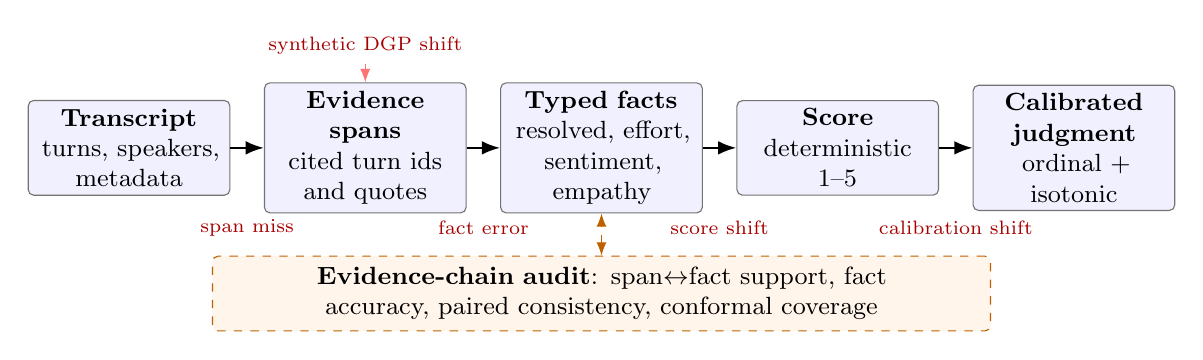
\begin{tikzpicture}[
  font=\small,
  >=Latex,
  stage/.style={draw=black!55, rounded corners=2pt, minimum height=1.15cm,
    text width=2.35cm, align=center, fill=blue!6, inner sep=3pt},
  audit/.style={draw=orange!75!black, dashed, rounded corners=2pt,
    fill=orange!8, align=center, text width=9.6cm, inner sep=4pt},
  fail/.style={font=\scriptsize, text=red!65!black, align=center},
  shiftlbl/.style={font=\scriptsize, text=red!65!black, align=center}
]
\node[stage] (t) at (0,0) {\textbf{Transcript}\\turns, speakers,\\metadata};
\node[stage] (s) at (3.0,0) {\textbf{Evidence spans}\\cited turn ids\\and quotes};
\node[stage] (f) at (6.0,0) {\textbf{Typed facts}\\resolved, effort,\\sentiment, empathy};
\node[stage] (sc) at (9.0,0) {\textbf{Score}\\deterministic\\1--5};
\node[stage] (cal) at (12.0,0) {\textbf{Calibrated}\\\textbf{judgment}\\ordinal + isotonic};

\draw[->, thick] (t) -- (s);
\draw[->, thick] (s) -- (f);
\draw[->, thick] (f) -- (sc);
\draw[->, thick] (sc) -- (cal);

\node[fail] at (1.5,-1.02) {span miss};
\node[fail] at (4.5,-1.02) {fact error};
\node[fail] at (7.5,-1.02) {score shift};
\node[fail] at (10.5,-1.02) {calibration shift};

\node[audit] (a) at (6.0,-1.85) {\textbf{Evidence-chain audit}: span$\leftrightarrow$fact support,
fact accuracy, paired consistency, conformal coverage};
\draw[<->, dashed, orange!75!black] (a.north) -- (f.south);

\node[shiftlbl] (shift) at (3.0,1.30) {synthetic DGP shift};
\draw[->, dashed, red!55] (shift.south) -- (s.north);
\end{tikzpicture}
\caption{The measurement chain and its failure loci. The same source-fitted extractor and
calibration layer are applied to each shifted target. The audit band is evaluated with both
oracle-assisted diagnostics (gold evidence turns) and label-free runtime flags.}
\label{fig:chain}
\end{figure}

\subsection{Synthetic data-generating process}

We generate 420 source calls: 240 train, 80 dev, and 100 sealed holdout. Each call has a persona
(anxious elderly, busy professional, angry returning, calm first-timer, vulnerable financial),
an issue type (billing, refund, technical, account access, cancellation), a resolution outcome
(resolved, partial, unresolved), caller effort (0--3), agent empathy (0/1), and an expressed
sentiment ($-2$ to $+2$). A structural equation combines resolution, empathy, effort, prior
failures, wait time, and persona into a latent satisfaction $z$; cutpoints map $z$ to a 1--5
latent label. A simulated post-call survey is a noisy draw around the latent label with about
71\% response; two simulated annotators provide noisy labels for a human-ceiling check.

The transcript is rendered from templates with explicit cue sentences for each fact. To avoid a
trivially perfect extractor, a fraction of cues is replaced by implicit but entailed evidence:
22\% of resolution cues, 18\% of empathy cues, 12\% of sentiment cues, and 10\% of effort cues.
Gold facts are unchanged; the information is still in the transcript, but the surface pattern is
gone. This creates realistic evidence scarcity without making the label unfair.

The deterministic score is a weighted sum of four normalised facts:
\begin{equation}
\mathrm{raw} = 1 + 4\cdot \operatorname{clip}\!\left(
0.55\,r + 0.20\,(1-e/3) + 0.15\,(s+2)/4 + 0.10\,a,\;0,\;1
\right),
\label{eq:score}
\end{equation}
where $r\in\{0,0.5,1\}$ is resolution, $e\in\{0,1,2,3\}$ is effort, $s\in[-2,2]$ is sentiment,
and $a\in\{0,1\}$ is empathy. The weights are transparent and fixed before any shift is
evaluated.

\subsection{Calibration and audit layers}

Calibration is fitted on source train+dev surveys only ($n=227$). We compare two layers: an
ordinal proportional-odds model on the raw score with a single temperature fitted on out-of-fold
predictions, and an isotonic regression of the survey label on the raw score
\citep{niculescu2005predicting}. The ordinal layer supplies class probabilities for ECE, Brier,
selective prediction, and conformal sets; isotonic supplies point scores. The implementation
uses scikit-learn for isotonic regression and the agreement metrics \citep{pedregosa2011scikit}. A split-conformal
layer uses nonconformity $1-p(y)$ and a 90\% target coverage \citep{angelopoulos2021gentle}; the
threshold is fitted on out-of-fold probabilities and applied unchanged to every target.

We report QWK \citep{cohen1968weighted}, mean absolute error, Spearman correlation, ECE
\begin{equation}
\ece = \sum_{b=1}^{B}\frac{n_b}{n}\left|\mathrm{acc}_b-\mathrm{conf}_b\right|,
\label{eq:ece}
\end{equation}
Brier score, negative log-likelihood, calibration slope (OLS of observed on predicted), the
large-error rate $P(|\hat y-y|>1)$, and conformal coverage/set size. All estimates carry 1,000
bootstrap resamples; paired shifts use paired $\Delta$QWK intervals. The source frame is the
sealed 100-call holdout; train/dev are never included in any reported target metric.

\subsection{Shift conditions}

Table~\ref{tab:shifts} summarises the five conditions. The first four are paired transformations
of the source holdout: the latent label and survey response are held fixed, so any change in the
score is attributable to the transformation. Persona mix is unpaired and changes the base rate.

\begin{table}[t]
\centering
\caption{Shift conditions. The first four are paired transformations of the source holdout:
latent satisfaction and survey response are held fixed. Persona mix is an unpaired covariate
shift with new calls.}
\label{tab:shifts}
\begin{threeparttable}
\begin{tabularx}{\textwidth}{@{}l X X@{}}
\toprule
Condition & Transformation & Intended stress \\
\midrule
Disfluency & Fillers, repetitions, and light ASR noise inside cue spans & Label-preserving measurement noise \\
Emotional arc & Late frustration after resolution, or suppressed dissatisfaction & Concept shift: expressed sentiment decouples from outcome \\
Paraphrase & Meaning-preserving synonym replacements for cue sentences & Lexical shift: tests span robustness \\
Combined & Paraphrase + emotional arc + disfluency & Realistic worst case \\
Persona mix & Different persona weights, new calls & Covariate shift / base-rate change \\
\bottomrule
\end{tabularx}
\begin{tablenotes}\footnotesize
\item All shifts are synthetic text transformations, not recordings of real disfluency, accent,
code-switching, or emotional expression.
\end{tablenotes}
\end{threeparttable}
\end{table}

\subsection{Hypotheses and decision rules}

We pre-specified four hypotheses. \textbf{H1} (calibration transfer): ECE increases and the
calibration slope departs from one under shift. \textbf{H2} (localisation): failures occur at the
span/fact layer before calibration, visible as a drop in gold evidence-turn hit rate or fact
accuracy while the latent label is unchanged. \textbf{H3} (audit signal): runtime evidence flags
predict large scoring errors better than posterior confidence by at least 0.05 AUC. \textbf{H4}
(conformal robustness): 90\% coverage falls below 0.85 under at least one shift. H3 and H4 are
deliberately falsifiable; a negative result is a finding.

Because the targets contain 100 calls, ECE intervals are wide. We therefore claim H1 only where
the paired $\Delta$QWK interval also excludes zero; otherwise the result is reported as
directional. This is a power constraint, not a post-hoc rescue.

\subsection{Direct LLM pilot}

To probe whether the evidence chain is the only way to score, we run a direct scorer: a local
\texttt{Qwen2.5-3B-Instruct-4bit} model \citep{qwen2024qwen25} via MLX, temperature 0, on 40
source-holdout calls and their paraphrase twins. The prompt asks for a 1--5 score, a five-class
distribution, verbalised confidence, cited turns, an exact quote, and a one-sentence rationale.
No calibration layer is fitted for this arm; the question is whether its raw scores and citations
are usable. This is a feasibility probe, not a frontier-model benchmark.

\section{Preliminary results}
\label{sec:results}

\subsection{Baseline and the survey ceiling}

Table~\ref{tab:baseline} reports the sealed source holdout. Against the latent construct, the
chain reaches QWK 0.718 and ECE 0.050, with a calibration slope close to one (0.985). Against
the noisy survey that the calibrator was actually fitted to, QWK falls to 0.502, ECE rises to
0.128, and the slope is 0.688. The large-error rate is 0.220 against latent and 0.384 against
survey.

\begin{table}[t]
\centering
\caption{Source holdout, $n=100$ (survey $n=73$). The calibration layer is fitted on train+dev
surveys only. QWK and ECE are evaluated against the generator's latent label and, separately,
against the simulated survey.}
\label{tab:baseline}
\begin{threeparttable}
\begin{tabular}{@{}lrr@{}}
\toprule
Metric & vs.\ latent & vs.\ survey \\
\midrule
QWK & 0.718 & 0.502 \\
Mean absolute error & 0.625 & 0.835 \\
ECE & 0.050 & 0.128 \\
Brier score & 0.625 & 0.737 \\
Calibration slope & 0.985 & 0.688 \\
Large-error rate & 0.220 & 0.384 \\
Conformal 90\% coverage & 0.976 & --- \\
\bottomrule
\end{tabular}
\begin{tablenotes}\footnotesize\raggedright
\item Bootstrap 95\% CI for source QWK vs.\ latent: $[0.605,0.802]$. The source conformal
coverage is above nominal because the base model is refit after the out-of-fold threshold;
coverage is therefore conservative on source.
\end{tablenotes}
\end{threeparttable}
\end{table}

This is the first audit finding. A service manager reading a survey-calibrated dashboard would
see a system that fits surveys reasonably; a researcher asking whether it measures satisfaction
would see a 0.216 QWK gap and a calibration slope of 0.688. Survey anchoring is not construct
validation.

\subsection{Shift profile}

Table~\ref{tab:shift} and Figure~\ref{fig:shift} give the main profile. Lexical paraphrase is
catastrophic: QWK 0.098, ECE 0.158, slope 1.341, large-error rate 0.440, conformal coverage
0.760. The combined shift is worse still: QWK 0.029, ECE 0.188, slope 0.019, large-error rate
0.590, coverage 0.750. Disfluency and emotional arc are milder (QWK 0.661 and 0.697; ECE 0.071
and 0.065), but their paired $\Delta$QWK intervals include zero:
$+0.057\,[-0.022,0.149]$ and $+0.021\,[-0.015,0.062]$. Only paraphrase
($+0.619\,[0.474,0.738]$) and combined ($+0.689\,[0.570,0.789]$) exclude zero. Persona mix is
not harmful on this draw (QWK 0.782), but it changes base rates and should not be read as
evidence of robustness.

\begin{table}[t]
\centering
\caption{Shift profile on the sealed source holdout and paired targets. QWK is against latent
satisfaction; ECE uses ordinal probabilities; coverage is 90\% split conformal. Brackets are
95\% bootstrap intervals for QWK; all intervals are wide at $n=100$.}
\label{tab:shift}
\begin{threeparttable}
\small
\begin{tabular}{@{}lcccccc@{}}
\toprule
Condition & QWK & 95\% CI & ECE & Slope & Large err. & Coverage \\
\midrule
Source & 0.718 & [0.605, 0.802] & 0.050 & 0.985 & 0.220 & 0.976 \\
Disfluency & 0.661 & [0.543, 0.754] & 0.071 & 1.040 & 0.280 & 0.980 \\
Emotional arc & 0.697 & [0.582, 0.783] & 0.065 & 1.018 & 0.270 & 0.970 \\
Paraphrase & 0.098 & [0.025, 0.191] & 0.158 & 1.341 & 0.440 & 0.760 \\
Combined & 0.029 & [$-$0.014, 0.082] & 0.188 & 0.019 & 0.590 & 0.750 \\
Persona mix & 0.782 & [0.693, 0.848] & 0.063 & 0.979 & 0.270 & 0.980 \\
\bottomrule
\end{tabular}
\begin{tablenotes}\footnotesize
\item ECE 95\% CIs overlap across source and the mild shifts (source $[0.031,0.164]$,
disfluency $[0.026,0.164]$, emotional arc $[0.032,0.168]$). The point estimates move in the
expected direction, but ECE alone does not separate the mild shifts from source at this sample
size.
\end{tablenotes}
\end{threeparttable}
\end{table}

\begin{figure}[t]
\centering
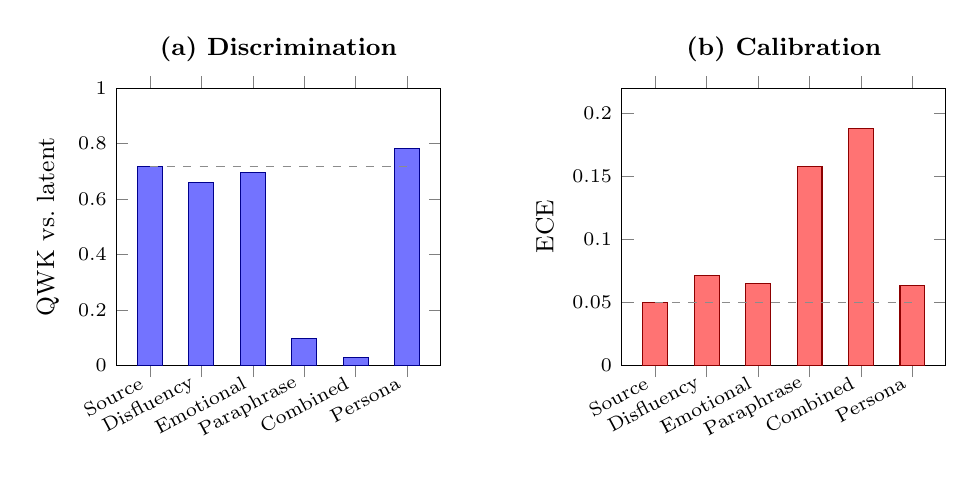
\begin{tikzpicture}
\begin{groupplot}[
  group style={group size=2 by 1, horizontal sep=2.3cm},
  width=0.47\textwidth, height=5.1cm,
  ybar,
  ymin=0, ymax=1,
  symbolic x coords={Source, Disfluency, Emotional, Paraphrase, Combined, Persona},
  xtick=data,
  x tick label style={rotate=28, anchor=east, font=\scriptsize},
  tick label style={font=\scriptsize},
  label style={font=\small},
  title style={font=\small\bfseries},
  enlarge x limits=0.13,
  scaled y ticks=false,
  yticklabel style={/pgf/number format/fixed},
]
\nextgroupplot[title={(a) Discrimination}, ylabel={QWK vs.\ latent}]
\addplot[fill=blue!55, draw=blue!55!black, bar width=9pt] coordinates {
  (Source,0.718) (Disfluency,0.661) (Emotional,0.697)
  (Paraphrase,0.098) (Combined,0.029) (Persona,0.782)};
\draw[dashed, black!45] (axis cs:Source,0.718) -- (axis cs:Persona,0.718);
\nextgroupplot[title={(b) Calibration}, ylabel={ECE}, ymax=0.22,
  ytick={0,0.05,0.10,0.15,0.20}]
\addplot[fill=red!55, draw=red!55!black, bar width=9pt] coordinates {
  (Source,0.050) (Disfluency,0.071) (Emotional,0.065)
  (Paraphrase,0.158) (Combined,0.188) (Persona,0.063)};
\draw[dashed, black!45] (axis cs:Source,0.050) -- (axis cs:Persona,0.050);
\end{groupplot}
\end{tikzpicture}
\caption{Shift profile. The dashed line marks the source value. QWK collapses under paraphrase
and combined shift; ECE rises, but its intervals overlap across the mild shifts (Table~\ref{tab:shift}).
The conformal coverage failure is sharper than the ECE change (Section~\ref{sec:evidence}).}
\label{fig:shift}
\end{figure}

\subsection{Where the chain breaks}
\label{sec:evidence}

Table~\ref{tab:evidence} localises the failure. Under paraphrase, the gold evidence-turn hit rate
falls from 0.848 to 0.082, the mean number of fact errors rises from 0.51 to 2.61, and quote
support falls to 0.260. Resolution accuracy is 0.190 and sentiment accuracy 0.360. The combined
shift is only slightly better on facts (2.54 errors) and quote support (0.690). Disfluency
degrades resolution accuracy to 0.650 and the gold-turn hit to 0.748 while sentiment accuracy
stays at 0.940. Emotional arc leaves resolution accuracy at 0.790 but drops sentiment accuracy
to 0.620 and produces a sentiment/resolution conflict on 38\% of calls.

\begin{table}[t]
\centering
\caption{Evidence-chain localisation. ``Gold turn hit'' is the fraction of facts whose cited turn
overlaps a generator cue turn. ``Quote supported'' checks that the extractor's quote appears in
the transcript. Both are oracle-assisted diagnostics, not deployable runtime flags.}
\label{tab:evidence}
\begin{threeparttable}
\small
\begin{tabular}{@{}lrrrrr@{}}
\toprule
Condition & Fact err. & Res.\ acc. & Sent.\ acc. & Gold hit & Quote sup. \\
\midrule
Source & 0.51 & 0.790 & 0.940 & 0.848 & 1.000 \\
Disfluency & 0.91 & 0.650 & 0.940 & 0.748 & 1.000 \\
Emotional arc & 0.83 & 0.790 & 0.620 & 0.867 & 1.000 \\
Paraphrase & 2.61 & 0.190 & 0.360 & 0.082 & 0.260 \\
Combined & 2.54 & 0.170 & 0.480 & 0.247 & 0.690 \\
Persona mix & 0.48 & 0.810 & 0.920 & 0.833 & 0.990 \\
\bottomrule
\end{tabular}
\begin{tablenotes}\footnotesize
\item Fact error is the mean number of incorrect facts (of four) per call. Oracle-assisted
columns use the generator's gold cue turns; the symbolic extractor is a lower bound, not an LLM.
\end{tablenotes}
\end{threeparttable}
\end{table}

The paired consistency results sharpen the claim. Under paraphrase, the average call changes
2.15 facts, 75\% of calls move the raw score by more than 0.5, 76\% change the predicted label,
and the evidence-turn Jaccard is 0.065---the cited turns are almost entirely different even
though the latent label is identical. Under disfluency the corresponding numbers are 0.43,
14\%, 23\%, and 0.915; under emotional arc they are 0.48, 0\%, 17\%, and 0.970. The lexical
shift is therefore a span-layer failure, not a gradual degradation of the same evidence.

The oracle repair confirms the localisation. A broad lexicon that adds the paraphrase synonyms
raises paraphrase QWK from 0.098 to 0.718 and the gold-turn hit from 0.082 to 0.848, with no
source change (0.718 to 0.718). But the repair was written by looking at the paraphrase list, so
it is an \emph{oracle upper bound}, not a deployable fix. Its value is diagnostic: if a known
synonym list recovers the chain, the failure is lexical, not a fundamental limit of fact-based
scoring.

\subsection{Calibration is not the bottleneck, but it is not enough}

The calibration layer behaves as designed on source: the ordinal model's temperature is 1.078,
the conformal threshold is 0.893, and the reliability curve is close to the diagonal against
latent. Under paraphrase, post-hoc isotonic calibration recovers QWK only to 0.107; the problem
is that the facts entering the calibrator are wrong or missing. Under combined shift the
calibration slope is 0.019---the score carries almost no signal about the latent construct.
Calibration cannot repair an evidence chain that has already broken upstream.

The survey-versus-latent gap is a second calibration lesson. A survey-anchored layer can improve
fit to the survey (isotonic QWK 0.549 vs.\ 0.502 raw on survey) while moving away from the
construct (isotonic QWK 0.717 vs.\ 0.718 raw on latent). The layer is doing what it was asked to
do; the question is whether the survey is the right target.

\subsection{Audit signals and the failed deferral policy}

Table~\ref{tab:audit} compares posterior confidence with three label-free flags for predicting
large errors. Posterior confidence is at or below chance for ranking large errors on source
(0.372), disfluency (0.275), and emotional arc (0.354). The missing-resolution flag beats
confidence on source (0.589 vs.\ 0.372), disfluency (0.624 vs.\ 0.275), and emotional arc
(0.648 vs.\ 0.354), but not on paraphrase (0.534 vs.\ 0.478) or combined (0.520 vs.\ 0.567).
The conflict flag is weak everywhere; the low-confidence flag is weak on source and paraphrase.

\begin{table}[t]
\centering
\caption{AUC for predicting a large error ($|\hat y-y|>1$) on latent satisfaction. Confidence is
the ordinal posterior maximum. Flags are label-free; ``missing res.'' is no cited resolution
evidence, ``conflict'' is a sentiment/resolution contradiction, ``low conf.'' is mean fact
confidence below 0.55.}
\label{tab:audit}
\begin{threeparttable}
\small
\begin{tabular}{@{}lrrrr@{}}
\toprule
Condition & Confidence & Missing res. & Conflict & Low conf. \\
\midrule
Source & 0.372 & 0.589 & 0.467 & 0.522 \\
Disfluency & 0.275 & 0.624 & 0.477 & 0.602 \\
Emotional arc & 0.354 & 0.648 & 0.426 & 0.525 \\
Paraphrase & 0.478 & 0.534 & --- & 0.494 \\
Combined & 0.567 & 0.520 & --- & 0.483 \\
Persona mix & 0.439 & 0.524 & 0.557 & 0.506 \\
\bottomrule
\end{tabular}
\begin{tablenotes}\footnotesize
\item AUC is a ranking diagnostic, not a deferral policy. The conflict flag is undefined when
no sentiment/resolution pair is extracted. These AUCs are exploratory and have no interval yet.
\end{tablenotes}
\end{threeparttable}
\end{table}

The deferral test is the decision-relevant check. A gate combining confidence with the three
flags improved the large-error rate at 80\% coverage by 0.0 pp (source), $-$2.5 pp (disfluency),
and $-$1.2 pp (emotional arc), but worsened paraphrase by +2.5 pp, and did not improve AUC
(max $\Delta$AUC $+0.015$). We discard it. The interpretation is that ``no evidence'' is often
the scorer's honest default, not the dangerous case; the dangerous case is \emph{confident wrong
evidence}. A presence flag cannot see that. A contradiction audit---does the cited span entail
the typed fact?---is the next candidate.

\subsection{Robustness versus auditability: the direct LLM contrast}

The direct 3B scorer is the most informative contrast in the pilot. On the same 40 source calls
and their paraphrase twins, the symbolic chain falls from QWK 0.746 to 0.113 under paraphrase,
while the direct LLM holds QWK at 0.669 to 0.667 (Table~\ref{tab:llm}, Figure~\ref{fig:llm}).
It also has a lower large-error rate (0.150 vs.\ 0.450 under paraphrase). But its five-class
probability ECE is 0.575 on source and 0.593 on paraphrase, its verbalised confidence averages
0.874 and 0.854, and its citation precision is 0.604 and 0.533. Its quotes are supported 95\%
and 90\% of the time, and cited turns hit a gold cue turn on 97.5\% and 92.5\% of calls, but
many of those turns are not the evidence for the score. The model is robust to vocabulary and
weakly auditable; the symbolic chain is auditable and brittle.

\begin{table}[t]
\centering
\caption{Direct 3B scorer versus the symbolic evidence chain on the same 40 source-holdout calls
and their paraphrase twins. ``Large error'' is $|\hat y-y|>1$; ECE is five-class probability ECE
for the direct arm and ordinal ECE for the symbolic arm.}
\label{tab:llm}
\begin{threeparttable}
\small
\begin{tabular}{@{}lrrrrrr@{}}
\toprule
Arm & Source QWK & Para.\ QWK & Source large & Para.\ large & Source ECE & Para.\ ECE \\
\midrule
Symbolic chain & 0.746 & 0.113 & 0.200 & 0.450 & 0.090 & 0.199 \\
Direct 3B LLM & 0.669 & 0.667 & 0.150 & 0.150 & 0.575 & 0.593 \\
\bottomrule
\end{tabular}
\begin{tablenotes}\footnotesize
\item Direct-arm audit: confidence ECE 0.498/0.478; mean confidence 0.874/0.854; citation
precision 0.604/0.533; quote support 0.95/0.90; parse rate 1.000/0.975. One local 3B model, 40
calls per condition, not a frontier-model result.
\end{tablenotes}
\end{threeparttable}
\end{table}

\begin{figure}[t]
\centering
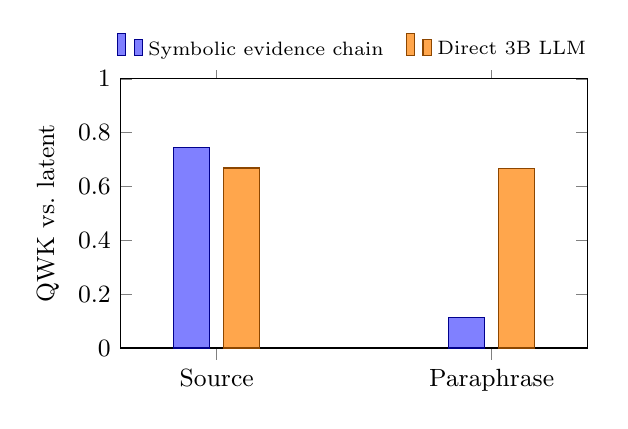
\begin{tikzpicture}
\begin{axis}[
  ybar=5pt,
  width=0.62\textwidth, height=5.0cm,
  ymin=0, ymax=1,
  symbolic x coords={Source, Paraphrase},
  xtick=data,
  ylabel={QWK vs.\ latent},
  tick label style={font=\small},
  label style={font=\small},
  legend style={at={(0.5,1.03)}, anchor=south, legend columns=2, draw=none,
    font=\scriptsize, /tikz/every even column/.append style={column sep=0.6em}},
  enlarge x limits=0.35,
]
\addplot[fill=blue!50, draw=blue!55!black, bar width=13pt] coordinates {(Source,0.746) (Paraphrase,0.113)};
\addplot[fill=orange!70, draw=orange!55!black, bar width=13pt] coordinates {(Source,0.669) (Paraphrase,0.667)};
\legend{Symbolic evidence chain, Direct 3B LLM}
\end{axis}
\end{tikzpicture}
\caption{The robustness--auditability contrast. The symbolic chain is more accurate on source and
collapses under paraphrase; the direct LLM is less accurate on source, stable under paraphrase,
and badly calibrated. The comparison uses the same 40 calls.}
\label{fig:llm}
\end{figure}

\subsection{What the preliminary evidence supports}

Table~\ref{tab:decisions} records the keep/discard decisions. Two are clear: broadening the
lexicon is a diagnostic upper bound, not a deployable fix; isotonic and ordinal calibration serve
different jobs and should both be kept. The runtime gate is discarded. The direct LLM is kept as
a pilot only.



The report's working claims, stated with the caveats they require, are:

\begin{enumerate}[leftmargin=1.4em,itemsep=0.3em]
\item \textbf{Lexical shift is an extractor-level failure, not a calibration-layer failure.}
The symbolic chain loses its spans (gold hit 0.848 $\rightarrow$ 0.082), post-hoc isotonic
recovers QWK only to 0.107, and the direct LLM holds QWK at 0.667. The fragile interface is
span/fact extraction.
\item \textbf{ECE is too blunt at this sample size.} Its point estimates rise in the expected
direction, but the source interval $[0.031,0.164]$ overlaps the mild-shift and paraphrase
intervals. Conformal coverage is sharper: 0.976 on source, 0.760 under paraphrase, 0.750 under
combined. An audit should report discrimination, evidence recovery, and coverage together.
\item \textbf{Survey anchoring is not construct validation.} The source chain reaches QWK 0.718
against latent but 0.502 against survey; ECE 0.050 vs.\ 0.128; slope 0.985 vs.\ 0.688.
\item \textbf{Evidence-presence flags are diagnostic, not a deferral policy.} Missing-resolution
AUC beats confidence on source, disfluency, and emotional arc, but the gate improves selective
risk in only two of four conditions and worsens paraphrase. The next audit should test
contradiction, not presence.
\item \textbf{Robustness and auditability trade off in this pilot.} The direct LLM is robust to
paraphrase but overconfident and weakly traceable; the symbolic chain is traceable but brittle.
The next design should put a robust extractor inside the auditable chain.
\end{enumerate}

\begin{table}[t]
\centering
\caption{Keep/discard ledger for the preliminary cycle.}
\label{tab:decisions}
\begin{tabularx}{\textwidth}{@{}l X l@{}}
\toprule
Card & Change & Decision \\
\midrule
C0 & Strict lexicon + source calibration (baseline) & Reference \\
C1 & Broad lexicon with paraphrase synonyms & Keep (diagnostic, circular) \\
C2 & Isotonic point calibration alongside ordinal probabilities & Keep both \\
C3 & Runtime evidence gate for abstention & Discard \\
C4 & Direct small-LLM scoring pilot & Pilot only \\
\bottomrule
\end{tabularx}
\end{table}

\section{Discussion}

The preliminary results suggest three shifts in how satisfaction scoring should be evaluated.

\paragraph{From score accuracy to evidence consistency.}
A QWK against a survey is a property of the score, not of the measurement chain. Two systems can
have the same QWK while one is supported by the right spans and the other by plausible-sounding
but wrong evidence. The paired design makes this visible: under paraphrase, 76\% of predicted
labels change even though the latent label is fixed, and the cited evidence turns are almost
entirely different (Jaccard 0.065). An audit that samples only scores will miss this; an audit
that samples spans will catch it.

\paragraph{From calibration error to a calibration profile.}
ECE is a useful summary but a poor sole trigger. In our pilot, ECE moves in the expected
direction under shift, yet its intervals overlap and it does not distinguish the mild shifts from
source. Conformal coverage, calibration slope, and the large-error rate give a fuller picture.
The broader lesson is consistent with the calibration-cliff literature
\citep{wang2026care}: post-hoc calibration is local to the distribution it was fitted on, and a
single number can hide the failure.

\paragraph{From presence to contradiction.}
The failed gate is informative. Missing evidence is often the scorer's honest default, and
therefore not a strong error signal. Confident wrong evidence is the dangerous case, and a
presence flag cannot detect it. A contradiction audit---checking whether the cited span entails
the typed fact---is a natural next step, and it aligns with evidence-boundary designs in
customer-service agents \citep{wu2026evidence}.

\paragraph{Implications for service governance.}
For ECIS Track 10, the practical implication is that synthetic-log-based satisfaction dashboards
need \emph{shift-aware} audits before they are used for coaching, compliance, or resource
allocation. The audit should be part of the measurement instrument, not an afterthought: which
spans support the score, does the score survive a meaning-preserving rewrite, and does the
calibration still cover under a plausible synthetic shift? The answers are governance-relevant
because they determine whether a manager is looking at satisfaction or at a survey-fitting
artefact.

\section{Threats to validity}
\label{sec:threats}

\paragraph{Synthetic ground truth.}
The latent label is a structural equation, not a human judgment. The survey is a noisy draw from
it, and the annotators are simulated. Every calibration number inherits that construction. The
design is useful for localising pipeline failures, not for estimating real-world CSAT accuracy.

\paragraph{Small targets and wide intervals.}
One hundred calls per shift gives QWK 95\% CIs of roughly $\pm0.06$--$0.10$. Only paraphrase and
combined have paired $\Delta$QWK intervals excluding zero. The disfluency and emotional-arc
effects are directional, not established. The next run should size targets for a paired effect
or report the mild shifts as inconclusive.

\paragraph{The offline extractor is a lower bound.}
It was written against the templates, so its source fact accuracy is optimistic and its
paraphrase collapse is partly a property of the lexicon. The broad-lexicon repair is circular by
construction. The direct LLM partially addresses this, but it is a scorer, not an extractor: the
evidence chain with an LLM extractor remains unrun.

\paragraph{The LLM pilot is small.}
One 3B open model, 40 calls per condition, a single prompt, temperature 0. It cannot rank models
or support a claim about GPT-class systems. Its value is to show that the audit instrument
transfers and that verbalised confidence is badly overconfident in this setting.

\paragraph{Synthetic transformations.}
The shifts operationalise Mirage-style dimensions, but they do not reproduce real disfluency,
accents, code-switching, or the full texture of emotional expression. The persona-mix target is
unpaired and changes base rates; its high QWK should not be read as robustness.

\paragraph{Calibration implementation.}
The conformal sets over-cover on source (0.976 vs.\ nominal 0.90) because the base model is
refit after the out-of-fold threshold. Coverage failures under shift are still informative, but
the source baseline is conservative. The 0.5 raw-score tolerance is coarse for sentiment-only
changes; label-change and expected-score deltas are therefore reported alongside it.

\section{Conclusion and next steps}

This report started a shift-aware audit of LLM-based satisfaction scoring on synthetic call
logs. The preliminary evidence is consistent with a simple claim: the calibration layer is not
the main source of fragility; the span/fact interface is. A known synonym list restores the
symbolic chain, and a direct 3B LLM is robust to the same paraphrase, but the direct model is
overconfident and only weakly traceable. Robustness and auditability trade off, and the next
design should combine them.

The immediate next experiments are:
\begin{enumerate}[leftmargin=1.4em,itemsep=0.25em]
\item Run a frontier LLM extractor through the typed-fact prompt on the same 100-call holdouts,
then score deterministically. Test whether it keeps the direct arm's paraphrase robustness while
retaining spans.
\item Add a contradiction audit: for each cited span, ask whether it entails the typed fact
(NLI or a second judge), and test whether contradiction rate predicts large errors better than
presence flags.
\item Run a frontier direct scorer with proper probability elicitation (verbalised histograms or
token logprobs) and temperature scaling on a source dev split.
\item Add a human-adjudicated subset (30--50 calls) to test whether the survey ceiling is an
artefact of the simulated annotators.
\item Pre-register the tolerance and the minimum detectable effect; the current 100-call targets
are underpowered for the mild shifts.
\end{enumerate}

\paragraph{Data and code.}
All data are synthetic and generated by the accompanying harness. The notebooks reproduce the
baseline, the shift profile, the audit, and the keep/discard ledger. The LLM pilot is optional and
requires the local model runtime.

\bibliographystyle{plainnat}
\bibliography{refs}

\end{document}
